\section{More on the Cross Product}
\label{sec:4_3}

The cross product $\vect{v} \times \vect{w}$ of two $\RR^3$-vectors $\vect{v} = \leftB
\begin{array}{r}
x_{1}\\
y_{1}\\
z_{1}
\end{array}
\rightB$ and $\vect{w} = \leftB
\begin{array}{r}
x_{2}\\
y_{2}\\
z_{2}
\end{array}
\rightB$
 was defined in Section~\ref{sec:4_2} where we observed that it can be best remembered using a determinant:\index{cross product!defined}\index{cross product!determinant form}\index{determinants!cross product}
\begin{equation} \label{eq:crossPdeterminant}
\vect{v} \times \vect{w} = \func{det}\leftB
\begin{array}{rrr}
\vect{i} & x_{1} & x_{2}\\
\vect{j} & y_{1} & y_{2}\\
\vect{k} & z_{1} & z_{2}
\end{array}
\rightB
=
\left|
\begin{array}{rr}
y_{1} & y_{2}\\
z_{1} & z_{2}
\end{array}
\right|\vect{i}
-
\left|
\begin{array}{rr}
x_{1} & x_{2}\\
z_{1} & z_{2}
\end{array}
\right|\vect{j}
+
\left|
\begin{array}{rr}
x_{1} & x_{2}\\
y_{1} & y_{2}
\end{array}
\right|\vect{k}
\end{equation}
Here $\vect{i} = \leftB
\begin{array}{r}
1\\
0\\
0
\end{array}
\rightB$, 
$\vect{j} = \leftB
\begin{array}{r}
0\\
1\\
0
\end{array}
\rightB$, and
$\vect{k} = \leftB
\begin{array}{r}
1\\
0\\
0
\end{array}
\rightB$ are the coordinate vectors, and the determinant is expanded along the first column. We observed (but did not prove) in Theorem \ref{thm:012164} that $\vect{v} \times \vect{w}$ is orthogonal to both $\vect{v}$ and $\vect{w}$. This follows easily from the next result.


\begin{theorem}{}{012676}
If 
$\vect{u} = \leftB
\begin{array}{r}
x_{0}\\
y_{0}\\
z_{0}
\end{array}
\rightB$,
$\vect{v} = \leftB
\begin{array}{r}
x_{1}\\
y_{1}\\
z_{1}
\end{array}
\rightB$, and 
$\vect{w} = \leftB
\begin{array}{r}
x_{2}\\
y_{2}\\
z_{2}
\end{array}
\rightB$, then 
$\vect{u} \dotprod (\vect{v} \times \vect{w}) = \func{det}\leftB
\begin{array}{rrr}
x_{0} & x_{1} & x_{2}\\
y_{0} & y_{1} & y_{2}\\
z_{0} & z_{1} & z_{2}
\end{array}
\rightB$.
\end{theorem}

\begin{proof}
Recall that $\vect{u} \dotprod (\vect{v} \times \vect{w})$ is computed by multiplying corresponding components of $\vect{u}$ and $\vect{v} \times \vect{w}$ and then adding. Using equation (\ref{eq:crossPdeterminant}), the result is:
\begin{equation*}
\vect{u} \dotprod (\vect{v} \times \vect{w}) 
= x_{0}\left(\left|
\begin{array}{rr}
y_{1} & y_{2}\\
z_{1} & z_{2}
\end{array}
\right|\right)
+ y_{0}\left(-
\left|
\begin{array}{rr}
x_{1} & x_{2}\\
z_{1} & z_{2}
\end{array}
\right|\right)
+z_{0}\left(
\left|
\begin{array}{rr}
x_{1} & x_{2}\\
y_{1} & y_{2}
\end{array}
\right|\right)
=
\func{det}\leftB
\begin{array}{rrr}
x_{0} & x_{1} & x_{2}\\
y_{0} & y_{1} & y_{2}\\
z_{0} & z_{1} & z_{2}
\end{array}
\rightB
\end{equation*}
where the last determinant is expanded along column 1.
\end{proof}

The result in Theorem~\ref{thm:012676} can be succinctly stated as follows: If $\vect{u}$, $\vect{v}$, and $\vect{w}$ are three vectors in $\RR^3$, then
\begin{equation*}
\vect{u} \dotprod (\vect{v} \times \vect{w}) = \func{det} \leftB \begin{array}{ccc} \vect{u} & \vect{v} & \vect{w}\end{array}\rightB
\end{equation*}
where $\leftB \begin{array}{ccc} \vect{u} & \vect{v} & \vect{w}\end{array}\rightB$ denotes the matrix with $\vect{u}$, $\vect{v}$, and $\vect{w}$ as its columns. Now it is clear that $\vect{v} \times \vect{w}$ is orthogonal to both $\vect{v}$ and $\vect{w}$ because the determinant of a matrix is zero if two columns are identical.


Because of (\ref{eq:crossPdeterminant}) and Theorem~\ref{thm:012676},
 several of the following properties of the cross product follow from 
properties of determinants (they can also be verified directly).

\begin{theorem}{}{012690}
Let $\vect{u}$, $\vect{v}$, and $\vect{w}$ denote arbitrary vectors in $\RR^3$.

\begin{multicols}{2}
\begin{enumerate}
\item $\vect{u} \times \vect{v}$ is a vector.

\item $\vect{u} \times \vect{v}$ is orthogonal to both $\vect{u}$ and $\vect{v}$.

\item $\vect{u} \times \vect{0} = \vect{0} = \vect{0} \times \vect{u}$.

\item $\vect{u} \times \vect{u} = \vect{0}$.

\item $\vect{u} \times \vect{v} = -(\vect{v} \times \vect{u})$.

\item $(k\vect{u}) \times \vect{v} = k(\vect{u} \times \vect{v}) = \vect{u} \times (k\vect{v})$ for any scalar $k$.

\item $\vect{u} \times (\vect{v} + \vect{w}) = (\vect{u} \times \vect{v}) + (\vect{u} \times \vect{w})$.

\item $(\vect{v} + \vect{w}) \times \vect{u} = (\vect{v} \times \vect{u}) + (\vect{w} \times \vect{u})$.

\end{enumerate}\index{cross product!properties of}
\end{multicols}
\end{theorem}

\begin{proof}
(1) is clear; (2) follows from Theorem~\ref{thm:012676};
 and (3) and (4) follow because the determinant of a matrix is zero if 
one column is zero or if two columns are identical. If two columns are 
interchanged, the determinant changes sign, and this proves (5). The 
proofs of (6), (7), and (8) are left as Exercise \ref{ex:ch4_3_ex15}. 
\end{proof}

\noindent We now come to a fundamental relationship between the dot and cross products.\index{cross product!and dot product}\index{dot product!and cross product}

\begin{theorem}{Lagrange Identity\footnotemark}{012715}
If $\vect{u}$ and $\vect{v}$ are any two vectors in $\RR^3$, then\index{Lagrange identity}\index{cross product!Lagrange Identity}
\begin{equation*}
\vectlength \vect{u} \times \vect{v} \vectlength^2 = \vectlength \vect{u} \vectlength^2\vectlength \vect{v} \vectlength^2 - (\vect{u} \dotprod \vect{v})^2
\end{equation*}
%\begin{figure}[H]
%\centering
%\includegraphics{4-vector-geometry/figures/3-more-on-the-cross-product/ufg04015}
%\caption{\label{fig:012721}}
%Photo \textcopyright  Corbis.
%\end{figure}
\end{theorem}
\footnotetext{Joseph
 Louis Lagrange\index{Lagrange, Joseph Louis} (1736--1813) was born in Italy and spent his early years 
in Turin. At the age of 19 he solved a famous problem by inventing an 
entirely new method, known today as the calculus of variations, and went
 on to become one of the greatest mathematicians of all time. His work 
brought a new level of rigour to analysis and his \textit{M\'{e}canique Analytique}\index{\textit{M\'{e}canique Analytique} (Lagrange)}
 is a masterpiece in which he introduced methods still in use. In 1766 
he was appointed to the Berlin Academy by Frederik the Great who 
asserted that the ``greatest mathematician in Europe'' should be at the 
court of the ``greatest king in Europe.'' After the death of Frederick, 
Lagrange went to Paris at the invitation of Louis XVI. He remained there
 throughout the revolution and was made a count by Napoleon.}

\begin{proof}
Given $\vect{u}$ and $\vect{v}$, introduce a coordinate system and write 
$\vect{u} = \leftB
\begin{array}{r}
x_{1}\\
y_{1}\\
z_{1}
\end{array}
\rightB$
and 
$\vect{v} = \leftB
\begin{array}{r}
x_{2}\\
y_{2}\\
z_{2}
\end{array}
\rightB$ in component form. Then all the terms in the identity can be computed 
in terms of the components. The detailed proof is left as Exercise ~\ref{ex:ch4_3_ex14}. 
\end{proof}

An expression for the magnitude of the vector $\vect{u} \times \vect{v}$ can be easily obtained from the Lagrange identity. If $\theta$ is the angle between $\vect{u}$ and $\vect{v}$, substituting $\vect{u} \dotprod \vect{v} = \vectlength\vect{u}\vectlength\vectlength\vect{v}\vectlength \cos \theta$ into the Lagrange identity gives
\begin{equation*}
\vectlength \vect{u} \times \vect{v} \vectlength^2 = \vectlength \vect{u} \vectlength^2\vectlength \vect{v} \vectlength^2 - \vectlength \vect{u} \vectlength^2\vectlength \vect{v} \vectlength^2\cos^2\theta = \vectlength \vect{u} \vectlength^2\vectlength \vect{v} \vectlength^2\sin^2\theta
\end{equation*}
using the fact that $1 - \cos^{2} \theta = \sin^{2} \theta$. But $\sin \theta$ is nonnegative on the range $0 \leq \theta \leq \pi$, so taking the positive square root of both sides gives
\begin{equation*}
\vectlength \vect{u} \times \vect{v} \vectlength = \vectlength \vect{u} \vectlength \vectlength \vect{v} \vectlength \sin\theta
\end{equation*}

\begin{wrapfigure}[7]{l}{6cm} 
\centering
\begin{tikzpicture}[scale=1.0]
\coordinate (origin) at (0, 0);
\coordinate (ptV) at (4, 0);

\draw[dkgreenvect, thick, -latex] (origin)-- +(60:2cm) node (ptU) {};
\path(origin)-- +(60:2cm) node[left, midway] {\small $\vect{u}$};
\draw[dkgreenvect, thick, -latex] (origin)--(ptV) node[below, text=black, midway] {\small $\vect{v}$};
\draw[dkbluevect, thick, dashed] (1, 0)--(ptU.center)-- ++(4, 0)--(ptV);
\draw[dkbluevect, thick] (1, 0.2)-- ++(0.2, 0)-- ++(0, -0.2);
\path(1, 0)--(ptU) node[right, midway] {\small $\vectlength\vect{u}\vectlength \sin \theta$};
\draw[dkbluevect, thick] (0.3, 0) arc [start angle=0,end angle=60,radius=0.3] node[right, text=black, pos=0.9] {\small $\theta$};

\end{tikzpicture}

\caption{\label{fig:012736}}
\end{wrapfigure}

This expression for $\vectlength\vect{u} \times \vect{v}\vectlength$
 makes no reference to a coordinate system and, moreover, it has a nice 
geometrical interpretation. The parallelogram determined by the vectors $\vect{u}$ and $\vect{v}$ has base length $\vectlength\vect{v}\vectlength$ and altitude $\vectlength\vect{u}\vectlength \sin \theta$ (see Figure~\ref{fig:012736}). Hence the area of the parallelogram formed by $\vect{u}$ and $\vect{v}$ is
\begin{equation*}
(\vectlength \vect{u} \vectlength \sin\theta) \vectlength \vect{v} \vectlength = \vectlength \vect{u} \times \vect{v} \vectlength
\end{equation*}

This proves the first part of Theorem~\ref{thm:012738}.


\begin{theorem}{}{012738}
If $\vect{u}$ and $\vect{v}$ are two nonzero vectors and $\theta$ is the angle between $\vect{u}$ and $\vect{v}$, then\index{area!parallelogram!equal to zero}\index{parallelogram!area equal to zero}


\begin{enumerate}
\item $\vectlength\vect{u} \times \vect{v}\vectlength = \vectlength\vect{u}\vectlength\vectlength\vect{v}\vectlength \sin \theta =$ the area of the parallelogram determined by $\vect{u}$ and $\vect{v}$.

\item $\vect{u}$ and $\vect{v}$ are parallel if and only if $\vect{u} \times \vect{v} = \vect{0}$.

\end{enumerate}
\end{theorem}

\begin{proof}[Proof of (2)]
By (1), $\vect{u} \times \vect{v} = \vect{0}$ if and only if the area of the parallelogram is zero. By Figure~\ref{fig:012736} the area vanishes if and only if $\vect{u}$ and $\vect{v}$ have the same or opposite direction---that is, if and only if they are parallel.
\end{proof}

\begin{example}{}{012749}

\begin{wrapfigure}[4]{l}{5cm} 
\vspace*{-1em}
\begin{tikzpicture}
\coordinate (ptP) at (-0.1, 2);
\coordinate (ptQ) at (3, 1);
\coordinate (ptR) at (0, 0);

\draw[dkgreenvect, thick] (ptP)--(ptQ)--(ptR)--cycle;
\draw[dkbluevect, thick, dashed] (ptP)-- ++(ptQ)--(ptQ);

\fill (ptP) circle (2pt);
\fill (ptQ) circle (2pt);
\fill (ptR) circle (2pt);

\node[left] at (ptP){\small $P$};
\node[right] at (ptQ){\small $Q$};
\node[left] at (ptR){\small $R$};
\end{tikzpicture}
%\captionof{figure}{\label{fig:012760}}
\end{wrapfigure}

\setlength{\rightskip}{0pt plus 200pt}
Find the area of the triangle with vertices $P(2, 1, 0)$, $Q(3, -1, 1)$, and $R(1, 0, 1)$.

\begin{solution}
We have 
$\longvect{RP} = \leftB
\begin{array}{r}
1\\
1\\
-1
\end{array}
\rightB$
 and 
$\longvect{RQ} = \leftB
\begin{array}{r}
2\\
-1\\
0
\end{array}
\rightB$. The area of the triangle is half the area of the parallelogram (see the diagram), and so equals $\frac{1}{2} \vectlength \longvect{RP} \times \longvect{RQ} \vectlength$. We have
\begin{equation*}
\longvect{RP} \times \longvect{RQ} = \func{det}\leftB
\begin{array}{rrr}
\vect{i} & 1 & 2\\
\vect{j} & 1 & -1\\
\vect{k} & -1 & 0
\end{array}
\rightB
=
\leftB
\begin{array}{r}
-1\\
-2\\
-3
\end{array}
\rightB
\end{equation*} so the area of the triangle is $\frac{1}{2} \vectlength \longvect{RP} \times \longvect{RQ} \vectlength = \frac{1}{2}\sqrt{1 + 4 + 9} = \frac{1}{2}\sqrt{14}.$

\end{solution}
\end{example}

\begin{wrapfigure}{l}{5cm} 
	\centering
	\begin{tikzpicture}[scale=0.9]
\coordinate (origin) at (0, 0);
\coordinate (ptV) at (3, 0);

\path (origin)--(-45:1cm) node (ptU) {};
\fill[ltbluevect] (origin)--(ptV)-- ++(-45:1cm)--(ptU.center)--cycle;

\draw[dkgreenvect, thick, -latex] (origin)--(45:1.5cm) node (ptW) {};
\draw[dkgreenvect, thick, -latex] (origin)--(ptV) node[below=0.005, text=black, pos=0.8] {\small $\vect{v}$};
\draw[dkgreenvect, thick, -latex] (origin)--(ptU.center);
\draw[dkgreenvect, thick, -latex] (origin)--(0, 1.5) node[right, text=black] {\small $\vect{u} \times \vect{v}$};

\draw[dkbluevect, thick, dashed] (ptW.center)-- ++(3, 0)-- ++(-45:1cm)-- ++(-3, 0) node (ptUPlusW) {} --cycle;
\draw[dkbluevect, thick, dashed] (ptUPlusW.center)--(ptU.center)-- ++(3, 0)-- ++(45:1.5cm);
\draw[dkbluevect, thick, dashed] (ptV)-- ++(45:1.5cm);
\draw[dkbluevect, thick, dashed] (ptV)-- ++(-45:1cm);

\draw[dkbluevect, thick] (ptW.center)-- ++(-90:1.25) node[right, midway] {\small $h$};

\path (origin)--(45:1.5cm) node[left, pos=0.7] {\small $\vect{w}$};
\path (origin)--(ptU.center) node[left, pos=0.6] {\small $\vect{u}$};
\end{tikzpicture}
	\caption{\label{fig:012763}}
\end{wrapfigure}

If three vectors $\vect{u}$, $\vect{v}$, and $\vect{w}$ are given, they determine a ``squashed'' rectangular solid called a \textbf{parallelepiped}\index{parallelepiped} (Figure~\ref{fig:012763}),
 and it is often useful to be able to find the volume of such a solid. 
The base of the solid is the parallelogram determined by $\vect{u}$ and $\vect{v}$, so it has area $A = \vectlength\vect{u} \times \vect{v}\vectlength$ by Theorem~\ref{thm:012738}. The height of the solid is the length $h$ of the projection of $\vect{w}$ on $\vect{u} \times \vect{v}$. Hence
\begin{equation*}
h = \left| \frac{\vect{w} \dotprod (\vect{u} \times \vect{v})}{\vectlength \vect{u} \times \vect{v} \vectlength^2}\right|\vectlength \vect{u} \times \vect{v} \vectlength = \frac{|\vect{w} \dotprod (\vect{u} \times \vect{v})|}{\vectlength \vect{u} \times \vect{v} \vectlength} = \frac{|\vect{w} \dotprod (\vect{u} \times \vect{v})|}{A}
\end{equation*}

Thus the volume of the parallelepiped is $hA = |\vect{w} \dotprod (\vect{u} \times \vect{v})|$\index{volume!of parallelepiped}. This proves


\begin{theorem}{}{012765}
The volume of the parallelepiped determined by three vectors $\vect{w}$, $\vect{u}$, and $\vect{v}$ (Figure~\ref{fig:012763}) is given by $|\vect{w} \dotprod (\vect{u} \times \vect{v})|$.
\end{theorem}

\begin{example}{}{012768}
Find the volume of the parallelepiped determined by the vectors
\begin{equation*}
\vect{w} = \leftB
\begin{array}{r}
1\\
2\\
-1
\end{array}
\rightB,
\vect{u} = \leftB
\begin{array}{r}
1\\
1\\
0
\end{array}
\rightB,
\vect{v} = \leftB
\begin{array}{r}
-2\\
0\\
1
\end{array}
\rightB
\end{equation*}
\begin{solution}
By Theorem~\ref{thm:012676}, 
$\vect{w} \dotprod (\vect{u} \times \vect{v}) = \func{det}\leftB
\begin{array}{rrr}
1 & 1 & -2\\
2 & 1 & 0\\
-1 & 0 & 1
\end{array}
\rightB = -3$.
Hence the volume is $|\vect{w} \dotprod (\vect{u} \times \vect{v})| = |-3| = 3$ by Theorem~\ref{thm:012765}.
\end{solution}
\end{example}

\begin{wrapfigure}[15]{l}{5cm}
\vspace*{-1em} 
\centering
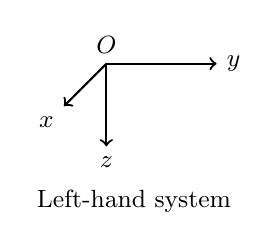
\begin{tikzpicture}[scale=0.7]
\coordinate (origin) (0, 0, 0);

\draw[thick, ->] (origin)--(2, 0, 0) node[right] {\small $y$};
\draw[thick, ->] (origin)--(0, -1.5, 0) node[below] {\small $z$};
\draw[thick, ->] (origin)--(0, 0, 2) node[below left] {\small $x$};
\node[above] (origin) {\small $O$};

\node at (0.5, -2.5, 0) {\small Left-hand system};
\end{tikzpicture}

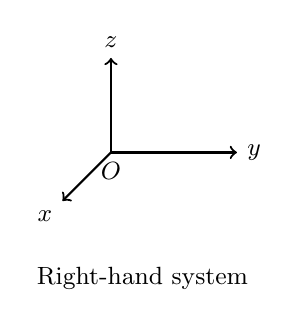
\begin{tikzpicture}[scale=0.8]
\coordinate (origin) (0, 0, 0);

\draw[thick, ->] (origin)--(2, 0, 0) node[right] {\small $y$};
\draw[thick, ->] (origin)--(0, 1.5, 0) node[above] {\small $z$};
\draw[thick, ->] (origin)--(0, 0, 2) node[below left] {\small $x$};
\node[below] (origin) {\small $O$};

\node at (0.5, -2, 0) {\small Right-hand system};
\end{tikzpicture}
\caption{\label{fig:012779}}
\end{wrapfigure}

We can now give an intrinsic description of the cross product $\vect{u} \times \vect{v}$. Its magnitude $\vectlength\vect{u} \times \vect{v}\vectlength = \vectlength\vect{u}\vectlength\vectlength\vect{v}\vectlength \sin \theta$ is coordinate-free. If $\vect{u} \times \vect{v} \neq \vect{0}$, its direction is very nearly determined by the fact that it is orthogonal to both $\vect{u}$ and $\vect{v}$ and so points along the line normal to the plane determined by $\vect{u}$ and $\vect{v}$. It remains only to decide which of the two possible directions is correct.\index{cross product!coordinate-free description}

Before this can be done, the basic issue of how coordinates are assigned must be clarified. When coordinate axes are chosen in space, the procedure is as follows: An origin is selected, two perpendicular lines (the $x$ and $y$ axes) are chosen through the origin, and a positive direction on each of these axes is selected quite arbitrarily. Then the line through the origin normal to this $x$-$y$ plane is called the $z$ axis, but there is a choice of which direction on this axis is the positive one. The two possibilities are shown in Figure~\ref{fig:012779}, and it is a standard convention that cartesian coordinates are always \textbf{right-hand coordinate systems}\index{right-hand coordinate systems}. The reason for this terminology is that, in such a system, if the $z$ axis is grasped in the right hand with the thumb pointing in the positive $z$ direction, then the fingers curl around from the positive $x$ axis to the positive $y$ axis (through a right angle).

Suppose now that $\vect{u}$ and $\vect{v}$ are given and that $\theta$ is the angle between them (so $0 \leq \theta \leq \pi$). Then the direction of $\vectlength\vect{u} \times \vect{v}\vectlength$ is given by the right-hand rule.


\begin{theorem*}[label=thm:012781]{Right-hand Rule}
If the vector $\vect{u} \times \vect{v}$ is grasped in the right hand and the fingers curl around from $\vect{u}$ to $\vect{v}$ through the angle $\theta$, the thumb points in the direction for $\vect{u} \times \vect{v}$.\index{cross product!right-hand rule}\index{right-hand rule}
\end{theorem*}

\begin{wrapfigure}[12]{l}{5cm} 
\centering
\begin{tikzpicture}[scale=1.0]
%set up of axis environment
\begin{axis}[view/h=110,disabledatascaling,
    width=5cm, 
    height=5cm, 
    xlabel={$x$}, 
    ylabel={$y$},
    zlabel={$z$},
    axis lines=center,
    axis on top=false,
    xtick=\empty,
    ytick=\empty,
    ztick=\empty,
    xticklabels=\empty, 
    yticklabels=\empty, 
    zticklabels=\empty, 
    every axis x label/.style={
      at={(ticklabel* cs:1.05)},
      anchor=north,
    },
    every axis y label/.style={
      at={(ticklabel* cs:1.05)},
      anchor=west,
    },
   every axis z label/.style={
      at={(ticklabel* cs:1.05)},
      anchor=south,
    },
    domain=0:5, 
    samples=100, 
    xmin=0, 
    xmax=4, 
    ymin=0, 
    ymax=5,
    zmin=0,
    zmax=1]

\coordinate (origin) at (0, 0, 0);
\coordinate (ptA) at (2, 0, 0);
\coordinate (ptB) at (3, 0, 0);
\coordinate (ptV) at (3, 4, 0);
\coordinate (ptC) at (0, 4, 0);

\draw[dkgreenvect, thick, -latex] (origin)--(ptV) node[above, text=black, pos=0.7] {\footnotesize $\vect{v}$};
\draw[dkbluevect, thick, dashed] (ptB)--(ptV)--(ptC);

\draw[dkbluevect, thick] (0.7, 0, 0) arc [start angle=0, end angle=53.13, radius=0.7] node[below, text=black, pos=0.9] {\footnotesize $\theta$};
\node[above] at (ptC) {\footnotesize $c$};
\node[above right] at (origin) {\footnotesize $O$};

\path (ptA)-- ++(0, 0.2, 0.05) node[left] {\footnotesize $a$};
\path (ptB)-- ++(0.0, -0.25, 0.02) node {\footnotesize $b$};

\draw[dkgreenvect, thick, -latex] (origin)--(ptA) node[right=0.05, text=black] {\footnotesize $\vect{u}$};
\end{axis}
\end{tikzpicture}

\caption{\label{fig:012789}}
\end{wrapfigure}

\noindent To indicate why this is true, introduce coordinates in $\RR^3$ as follows: Let $\vect{u}$ and $\vect{v}$ have a common tail $O$, choose the origin at $O$, choose the $x$ axis so that $\vect{u}$ points in the positive $x$ direction, and then choose the $y$ axis so that $\vect{v}$ is in the $x$-$y$ plane and the positive $y$ axis is on the same side of the $x$ axis as $\vect{v}$. Then, in this system, $\vect{u}$ and $\vect{v}$ have component form 
$\vect{u} = \leftB
\begin{array}{r}
a\\
0\\
0
\end{array}
\rightB$
and 
$\vect{v} = \leftB
\begin{array}{r}
b\\
c\\
0
\end{array}
\rightB$
 where $a > 0$ and $c > 0$. The situation is depicted in Figure~\ref{fig:012789}. The right-hand rule asserts that $\vect{u} \times \vect{v}$ should point in the positive $z$ direction. But our definition of $\vect{u} \times \vect{v}$ gives
\begin{equation*}
\vect{u} \times \vect{v} = \func{det}\leftB
\begin{array}{rrr}
\vect{i} & a & b\\
\vect{j} & 0 & c\\
\vect{k} & 0 & 0
\end{array}
\rightB = 
\leftB
\begin{array}{c}
0\\
0\\
ac
\end{array}
\rightB = (ac)\vect{k}
\end{equation*}
and $(ac) \vect{k}$ has the positive $z$ direction because $ac > 0$.
